\documentclass{book}
%\input{latexmacro}
\usepackage{Sweave}
\usepackage{verbatim}
\usepackage{graphicx}
\usepackage{amsmath}
\usepackage{amssymb}
%\usepackage{hyperref}
\DeclareMathOperator*{\E}{\mathbb{E}}
\begin{document}
\input{RSim-concordance}
\setcounter{chapter}{3}


% special version of Chapter 4 for Louis to edit to create R version based on simmer
% 6/9/2012  6/26/2012  6/27/2012  7/2/2012
% definitions added just for this version
% Further used as a starting point by 
\newtheorem{example}{Example}[chapter]
\def\ttf{\texttt{TTF}}
\def\Clock{\texttt{Clock}}
\def\Entity{\textttf{Entity}}
\def\D{\mathrm{d}}
\def\yield{\texttt{yield}}
\def\EventNotice{\texttt{EventNotice}}
%\def\Process{\texttt{Process}}
%\def\Resource{\texttt{Resource}}
\def\Level{\textbf{Level}}
\def\Store{\textbf{Store}}
\def\Monitor{\textbf{Monitor}}
\def\Tally{\textbf{Tally}}
% end special definitions

\chapter{Simulation Programming with R and Simmer}

\label{ch:rsim}
\index{R}
\index{simmer}

This chapter shows how simulations of some of the examples in
Chapter 3  can be programmed using R and the Simmer simulation library\cite{simmer2016}\footnote{by Louis Luangkesorn <louis.luangkesorn@gmail.com>. This is intended to be an appendix to \cite{Nelson2013} which can be obtained at http://users.iems.northwestern.edu/~nelsonb/IEMS435/.  These language supplements replace Chapter 4 in that book.}. 
The goals of the chapter are to introduce R and Simmer, and to hint at the experiment design and analysis issues that will be covered in later chapters. %Chap. 3 {%~\ref{ch:examples}}
While this chapter will generally follow the flow of Chap. 4 from the main text, it will use the conventions and patterns enabled by the Simmer library instead of the event-scheduling approach of VBASim.


\section{Simmer Overview}
\label{sec:simmer.overview}

Simmer is process-based discrete-event simulation library for R \cite{rcoreteam2016a}. It is open source and released under the MIT license.  Simmer provides the modeler with components of a simulation model including processes, for active components like customers, messages, and vehicles, and resources, for passive components that form limited capacity congestion points like servers, checkout counters, and tunnels. It also provides monitor facilities to aid in gathering and reporting simulation statistics.

While Simmer comes with data collection capabilities, it depends on other R libraries for data analysis and reporting.
Common tasks include data analysis, reporting, and graphical display. 
Many data analysis oriented libraries use the {\em data frame} data type, which combines features of matrices and lists. Among the advantages of data frames is that it maintains the relationship between the variables that describe observations. Data analysis libraries that use data frames can take advantage of efficient processing of data even when variables have different data types (e.g. numeric values and categorical or text values.)

Some standard libraries include {\tt tidyr} \cite{wickham2014} for organizing data into data frames, {\tt dplyr} \cite{wickham2015} for manipulating data frames, and {\tt ggplot} \cite{wickham2009} for a wide range of plots and charts. 

Other useful functions and libraries include those for importing data from text files, csv files, relational databases, or from file formats associated with propriatary software packages such as SAS, SPSS, or Microsoft Excel. \cite{rcoreteam2016b}. 
A good starting place for learning how to use R for data analysis is the R for Data Analysis by Hadley Wickham \footnote{http://r4ds.had.co.nz/}.

To install Simmer, use the Packages -> Install feature of your Integrated Development Environment (IDE, such as RStudio \footnote{https://www.rstudio.com/products/rstudio/}) or enter the following in the R console:

\begin{verbatim}
install.packages("simmer")
\end{verbatim}

If you have not done so before, you may be asked to choose a nearby Comprehensive R Archive Network (CRAN) server from a list of servers around the world.

The other required libraries can be installed in a similar manner.  See the specific library webpages for more information.

This chapter will assume that you have {\tt dplyr}, {\tt magrittr} and {\tt ggplot2} packages installed. 

For an introduction to simmer, the best resource are the vignettes that are present with the documentationof the higher quality packages. They can be accessed by finding simmer in the installed packages (or in the Packages section of your IDE), or on CRAN 
\footnote{https://cran.r-project.org/web/packages/simmer/vignettes/A-introduction.html}.

Because simmer heavily utilizes the pipe operator, {\tt \%>\%}, it will be useful to review the use of the pipe operator from the magrittr package \footnote{https://cran.r-project.org/web/packages/magrittr/vignettes/magrittr.html}.

\subsection{Random numbers}

Because R is primarily used by statisticians, a wide range of probability distributions and functions for using those distributions are built into R. A starting point for a list of distributions and their use is in Introduction to R \footnote{https://cran.r-project.org/doc/manuals/r-release/R-intro.html\#Probability-distributions}.

For each probability distribution, there are four R functions that are used to access the distribution.

\begin{enumerate}
  \item Density function - {\tt dxxx} - The density of the probability distribution at a given point.
  \item Probability function - {\tt pxxx} - The cumulative probability distribution at a given point.
  \item Quantile function - {\tt qxxx} - The value that corresponds to a given quantile for the distribution.
  \item Random deviate - {\tt rxxx} - a random draw from a given distribution.
\end{enumerate}

Most commonly used in simulation is the random number generation function.  
Each distribution requires certain parameters to specify the distribution.
Then, the {\tt rxxx} function draws from that random variable.
For example, the exponential distribution is given the R name {\tt exp}, so the function to generate a random variate is {\tt rexp}. 
Using the command {\tt help rexp} tells you that the required parameters are the number of observations required and that the exponential distribution is parameterized by the rate.

{\tt rexp(n, rate = 1)}

Similarly, for the normal distribution, its name in R is {\tt norm}, so the function to generate a random variate is:

{\tt rnorm(n, mean = 0, sd = 1)}


As you already know, the pseudorandom number generators used to create
random variates in simulations essentially create a long list.
Random-number streams are just different starting places in this
list, spaced far apart. 
The need for streams is discussed in Chap. 7,%~\ref{ch:output},
but it is important to know that any stream is as good as any other stream
in a well-tested generator. \index{random-number stream}
In R, the random number stream used is set using the seed functions (\texttt{set.seed(seed)}), with an integer arguement to provide for reproducability and for blocking in design of experiments.

The following Time to Failure simulation is taken from Chapter 2. This represents a process with two machines where one machine is required and there is one machine for a backup. When a machine fails, the other machine takes over while the first machine is being repaired.  A system failure occurs when both machines are down at the same time (i.e. the second failure occurs before the first is repaired.)

\begin{figure}[tbp]
\begin{minipage}[t]{6in}\small
\begin{verbatim}

failure <- function(sinit, s, slast, clock, tlast, area){
  # A failure is occurring
  s = s-1
  if (s > 0)
    NextFailure = clock + sample(1:6,1)
  # Scheduling the next failure
  if (s == (Sinit - 1))
    NextRepair = clock + 2.5
  # Scheduling the next repair since there is no repair ongoing
  area = area + slast * (clock - tlast)
  tlast = clock
  slast = s
  state <- list(s=s, NextFailure=NextFailure, NextRepair=NextRepair, area=area)
}

repair <- function(sinit, s, slast, clock, tlast, area){
  # A repair completed
  s = s+1
  if (s < sinit)
    NextRepair = clock + 2.5
  else
    NextRepair = clock + 1000000
  area = area + slast * (clock - tlast)
  tlast = clock
  slast = s
  state <- list(s=s, NextFailure=NextFailure, NextRepair=NextRepair, area=area)
}

timerfunc <- function(NextFailure, NextRepair, sinit, s, slast, clock, tlast, area){
  if (NextFailure < NextRepair){
    timer = "Failure"
    clock = NextFailure
    NextFailure = 1000000
  } else {
    timer = "Repair"
    clock = NextRepair
    NextRepair = 1000000
  }
  ret <- list(s=s, NextFailure = NextFailure, NextRepair = NextRepair, 
              timer = timer, clock = clock)
}
\end{verbatim}
\end{minipage}
\caption{Time to failure event functions in R.}
\label{fig:ttfrevents}
\end{figure}

In the Time to Failure simulation in Figure \ref{fig:ttfrevents}, there are three processes represented as functions: Failure, Repair, and a timer function that tracks the simulation clock. 

Each function updates the state of the system then returns the result as a list. This is necessary as R functions can only return a single value.  This is the last line of the the {\tt Failure} and {\tt Repair} functions.


{\tt state <- list(s=s, NextFailure=NextFailure, \\ NextRepair=NextRepair, area=area)}

In the main part of the simulation (Figure \ref{fig:ttfrmain}), the results are accessed through the {\tt state\$value} pattern

{\tt NextFailure=state\$NextFailure}

The {\tt timerfunc} function updates the simulation clock. When called, it checks the current event as specified in the {\tt timer} variable, either "Failure" or "Repair", then updates the clock and state variables as appropriate.

\begin{figure}[tbp]
\begin{minipage}[t]{6in}\small
\begin{verbatim}

TTF <- function(aseed){
  set.seed(aseed)
  print("We are beginning the TTF simulation!")
  s = Sinit
  clock = 0
  NextFailure = sample(1:6, 1)
  NextRepair = 1000000
  slast = s
  tlast = 0
  area = 0
  timer = "Failure"
  while(s > 0){
    cat("At time ", clock)
    cat(" we have ", s, " machines operating", "\n")
    #list[s, NextFailure, NextRepair, timer, clock] <- 
    ret <- 
      timerfunc(NextFailure, NextRepair, Sinit, s, slast, clock, tlast, area)
    if(ret$timer=="Failure"){
      cat("there is a failure occurring at time ", ret$clock, "\n")
      state <- 
        failure(Sinit, ret$s, slast, ret$clock, tlast, ret$area)
      cat("Next failure is at ", state$NextFailure)
    } else {
      if (ret$timer=="Repair"){
        cat("there is a repair completed at time ", ret$clock, "\n")
            state <- 
              repair(Sinit, ret$s, slast, ret$clock, tlast, ret$area)
      } else{
        print("Done!")
        print(ret$clock)
      }
      
    }
    NextFailure=state$NextFailure
    NextRepair = state$NextRepair
    s=state$s
    area=ret$area
    clock = ret$clock
  }
  taverage = area/clock
  print("There are no machines left!")
  print("The time of failure is ", clock)
  print("The average number of components was ", taverage)
  list(taverage, clock)
}
TTF(123)

\end{verbatim}
\end{minipage}
\caption{Time to failure main function in R.}
\label{fig:ttfrmain}
\end{figure}


The {\tt TTF} function is the main function of the simulation.  It takes the random number seed for the current run of the simulation as an arguement. This enables the simulation analyst to reproduce the results of the simulation.  Next, the simulation initializes state variables, reporting variables, and the simulation clock.  The main loop of the simulation uses the simulation clock to determine the next event, then calls the appropriate event routine which will update the system state, 

While a simple system like this two machine system can be modeled in R directly, more complex systems are better modeled using a simulation library that provides many of the accounting details of simulation and a shorthand for specifying the model.  For R, the {\tt simmer} package provides this.

\subsection{Simmer components}

The {\tt simmer} package was developed as a simple rapid development discrete event simulation (DES) framework that had the analysis and plotting capabilities of R readily available. \cite{Simmer2016}

A simmer simulation program has two parts. First is the simulation itself, which creates resources and generates entities. The other part are the trajectories, which define how entities move between the available resources in the simulation.

The main simulation routine identifies the simulation and the resources and entities.

\begin{figure}[tbp]
\begin{minipage}[t]{6in}\small
\verbatiminput{carcharge.R}
\end{minipage}
\caption{Car charging example using simmer.}
\label{fig:carcharge}
\end{figure}

The first code block initializes variables required throughout the simulation.  For simplicity, these are declared as global variables.

Next, the simulation object is created using {\tt simmer()}.

As Simmer is a process based DES, the simulation defines each process using {\tt create\_trajectory()}.
Each trajectory has a name, then uses the {\tt \%>\%} construct to define each step that would be experienced by a trajectory of that type. \footnote{Detailed information on trajectories can be found at {\em Advanced Trajectory Usage} https://cran.r-project.org/web/packages/simmer/vignettes/C-trajectories.html}.
The trajectory includes steps such as seizing {\tt seize()} and releasing {\tt release()} resources, and how long a wait should be before the next step (e.g how long a resource is used in this process).

After the simulation is created and the trajectories defined, the simulation itself is defined.
Using the {\tt \%>\%} construct again, the simulation {\tt add\_resource}, which includes the name of the resource (to be used in all trajectories), the capacity, and if Simmer should have a monitor to collect resource usage.
The simulation will also generate entities that will follow specific trajectories using {\tt add\_generator()}.  The call to {\tt add\_generator} will include the name of the process generating entities, the trajectory that those entities will follow, and the inter-arrival process of the generator. In this case, the interarrival process ({\tt sample()}) is a function that draws a random integer indicated the number of periods before the next arrival.

The simulation itself is run using the {\tt run()} command. 
{\tt run()} is applied using the {\tt \%>\%} construct and can include a stopping condition such as the time to end the simulation, {\tt until=c(160)}.

Last is reporting.
{\tt env \%>\% get\_mon\_resources()} displays the output of the resource monitors.
This output can be directed towards an output file, or into a data frame for further analysis or for output into structured forms such as spreadsheets or database tables using appropriate R libraries.


\section{Simulating the $M(t)/M/\infty$ Queue}
\label{sec:sim.mminf}

Here we consider the parking lot example of Sect.~3.1%\ref{sec:mminf},
a queueing system with time-varying car arrival rate, exponentially
distributed parking time and an infinite number of parking spaces.

A Simmer simulation generally consists of import of libraries, defining processes or trajectories that will be followed by entities, setting parameters, a main simulation program specifying resources and entity generators, and finally reporting.

At the top of the program are the libraries modules used.  (Fig.~\ref{fig:parking.import})
In addition to {\tt simmer}, these are the {\tt ggplot2} plotting library and the {\tt dplyr} library for data manipulation.


\begin{figure}[tbp]
\begin{minipage}[t]{6in}\small
\begin{verbatim}
library(simmer)
library(simmer.plot)
library(ggplot2)
library(dplyr)
set.seed(1234)
parkingtime = 2
\end{verbatim}
\end{minipage}
\caption{Library imports.}
\label{fig:parking.import}
\end{figure}


Next are two components, the cars and the arrival process. (Fig.~\ref{fig:parking.components})
The {\tt create\_trajectory} construction creates an instance of an entity that follows the {\em Car path} through the system. In this case, it seizes a parking spot for a period of time that is drawn from an exponential distribution.
The car then releases the parking spot as it leaves.

\begin{figure}[tbp]
\begin{minipage}[t]{6in}\small
\begin{verbatim}
env <- simmer("ParkingSimulation")

arrival <- trajectory("Car path") %>%
  seize("parking", 1) %>%
  timeout(function() rexp(1, 1/parkingtime)) %>%
  release("parking", 1)

env %>%
  add_resource("parking", capacity = 100, mon=TRUE) %>%
  add_generator("arrival", arrival, function() rexp(1, 25))

env %>% run(until= (24))

head(
  env %>% get_mon_resources()
)

plot(get_mon_resources(env), metric="usage")
\end{verbatim}
\end{minipage}
\caption{Parking resources and entity generators \label{fig:parking.components}}
\end{figure}

To define the simulation, you define the resources and generate the entities that will go into the simulation. In Figure \ref{fig:parking.components} these are the 100 parking spaces and the cars that arrive at a rate of 25/hour.
The parking lot is monitored to collect statistics on resource usage.
The {\em plot(get\_mon\_resources(env), metric="usage")} function plots the resource (parking lot) usage over time for this iteration.

This results in the plot in Fig.~\ref{fig:parkedcars.plot}.
Note that the horizontal dotted line at the top is the number of servers (parking spaces), the jagged line is the instantaneous number of parked cars, and the smooth line is the average utilization at that point in time.

\begin{figure}[tbp]
\centerline{\includegraphics[width=4in]{figures/parkedcars}}
\caption{Number of parked cars over time.}
\label{fig:parkedcars.plot}
\end{figure}

To make inferences or conclusions based on the simulation, it is necessary to run the simulation many replications.  So to find the daily average of the number of cars, we can run the simulation over 1000 days and look at the average and maximum parking over that period.  Fig.~\ref{fig:parking.replications} shows how to do this using a \texttt{for} loop.  
For each replication, initialize the \texttt{parkinglot} instance of the simulation object, then \texttt{run} using a new random number seed.

\begin{figure}[tbp]
\begin{minipage}[t]{6in}\small
\begin{verbatim}
envs <- lapply(1:100, function(i) {
  simmer("ReplicatedParkingSim") %>%
    add_resource("parking", 100) %>%
    add_generator("arrival", arrival, function() rexp(1, 25)) %>% 
    run(until= (24))
})

plot(get_mon_resources(envs), metric = "utilization")
\end{verbatim}
\end{minipage}
\caption{Running 100 replications}
\label{fig:parking.replications}
\end{figure}

Finally, {\tt plot(get\_mon\_resources(envs), metric = "utilization")} plots the average and 95\% confidence intervals of the parking lot utilization across the 100 replications using a box plot (Figure \ref{fig:parkedcars.utilization}).

\begin{figure}[tbp]
\centerline{\includegraphics[width=4in]{figures/ParkingUtilization}}
\caption{Parking lot utilization over 24 hour replications.}
\label{fig:parkedcars.utilization}
\end{figure}

\subsection{Issues and Extensions}
\label{sec:sim.mminf.issues}

\begin{enumerate}

\item The $M(t)/M/\infty$ simulation presented here simulates $24$
hours of parking lot operation, and treats each $24$-hour period
as as independent replication starting with an empty garage. This only
makes sense if the garage is emptied each day, for instance if the
mall closes at night. Is the assumed arrival rate $\lambda(t)$
appropriate for a mall that closes at night?

\item Suppose that the parking lot serves a facility that is
actually in operation $24$ hours a day, seven days per week (that is,
all the time). How should the simulation be initialized, and how long
should the run length be in this case?

\item How could the simulation be initialized so that there are $100$
cars in the parking lot at time $0$? 

\item When this example was introduced in Sect.~3.1 %\ref{sec:mminf}
, it was suggested that we size the garage based on the (Poisson)
distribution of the number of cars in the garage at the point in time
when the mean number in the garage was maximum. Is that what we did,
empirically, here? If not, how is the quantity we estimated by
simulation related to the suggestion in Sect.~3.1%\ref{sec:mminf} 
(for instance, will the simulation tend to suggest a bigger or smaller
garage than the analytical solution in Sect.~3.1%\ref{sec:mminf})?

\item One reason that this
simulation executes quite slowly when $\lambda(t) = 1000 +
100\sin(\pi t/12)$ is that the thinning method we used is very
inefficient (lots of possible arrivals are rejected). Speculate about
ways to make it faster.

\item For stochastic processes experts: Another reason that the
simulation is slow when $\lambda(t) = 1000 + 100\sin(\pi t/12)$ is
that there can be $1000$ or more pending departure events in the event list at any time, 
which means that scheduling a new event in
chronological order involves a slow search. However, it is possible
to exploit the memoryless property of the exponential distribution of
parking time to create an equivalent simulation that has only two
pending events (the next car arrival and next car departure) at any
point in time. Describe how to do this.

\end{enumerate}


\section{Simulating the $M/G/1$ Queue}
\label{sec:sim.mg1}

Here we consider the hospital example of Sect.~3.2,%\ref{sec:mg1}
a queueing system with Poisson arrival process, some (as yet
unspecified) service-time distribution, and a single server (either a
receptionist or an electronic kiosk); in other words, an $M/G/1$
queue.\index{$M/G/1$ queue} Patient waiting time is the key system
performance measure, and the long-run average waiting time in
particular.

Recall that Lindley's Equation~(3.3) % (\ref{eq:lindley}) 
provides a shortcut
way to simulate  successive customer waiting times:\index{Lindley's Equation}
\begin{eqnarray*}
Y_0 &=& 0 \qquad X_0 = 0 \\
Y_i &=& \max\{0, Y_{i-1} + X_{i-1} - A_i\},\ i=1,2,\ldots
\end{eqnarray*}
where $Y_i$ is the $i$th customer's waiting time, $X_i$ is that
customer's service time, and $A_i$ is the interarrival time between
customers $i-1$ and $i$. Lindley's equation avoids the need for an
event-based simulation, but is limited in what it produces (how would
you track the time-average number of customers in the queue?). In
this section we will describe both recursion-based and event-based
simulations of this queue, starting with the recursion.

\subsection{Lindley Simulation of the $M/G/1$ Queue}
\label{sec:sim.mg1.lindley}

To be specific, suppose that the mean time between arrivals is $1$
minute, with the distribution being exponential, and the mean time to use
the kiosk is $0.8$ minutes ($48$ seconds), with the distribution
being an Erlang-$3$.\index{Erlang distribution} An Erlang-$p$ is the
sum of $p$ i.i.d.\ exponentially distributed random variables, so an
Erlang-$3$ with mean $0.8$ is the sum of $3$ exponentially
distributed random variables each with mean $0.8/3$.

In Sect.~3.2 %\ref{sec:mg1} 
we noted that the waiting-time
random variables $Y_1, Y_2, \ldots$ converge in distribution to a
random-variable $Y$, and it is $\mu = \E(Y)$ that we will use to
summarize the performance of the queueing system. We also noted that
$\bar{Y}(m) = m^{-1}\sum_{i=1}^m Y_i$ converges with probability $1$
to $\mu$ as the number of customers simulated $m$ goes to infinity.

All of this suggests that we make a very long simulation run (large
$m$) and estimate $\mu$ by the average of the observed waiting times
$Y_1, Y_2, \ldots, Y_m$. But this is not what we will do, and here is
why: Any $m$ we pick is not $\infty$, so the waiting times early in
the run---which will tend to be smaller than $\mu$ because
the queue starts empty---will likely pull $\bar{Y}(m)$ down. To
reduce this effect, we will let the simulation generate waiting times
for a while (say $d$ of them) before starting to actually include
them in our average. We will still make $m$ large, but our average
will only include the last $m-d$ waiting times. That is, we will use as
our estimator the truncated average \index{truncated average}
\begin{equation}
\label{eq:truncated.average}
\bar{Y}(m,d) = \frac{1}{m-d}\sum_{i=d+1}^m Y_i .
\end{equation}
In addition, we will not make a single run of $m$ customers, but
instead will make
$n$ replications. This yields $n$ i.i.d.\ averages $\bar{Y}_1(m,d),
\bar{Y}_2(m,d),
\ldots, \bar{Y}_{n}(m,d)$ to which we can apply standard statistical
analysis. This avoids the need to directly estimate the asymptotic
variance $\gamma^2$, a topic we defer to later chapters.

\begin{figure}[tbp]
\begin{verbatim}
lindley <- function(m=55000, d=5000){
  replications <- 10
  lindley <- c()
  for (rep in 1:replications){
    y<- 0
    SumY <- 0
    for (i in 1:d){
      a <- rexp(1,1)
      x <- rgamma(1, shape=3, scale = 0.8/3)
      y <- max(0, y + x -a)
    }
    for (i in d:m){
      a <- rexp(1,1)
      x <- rgamma(1, shape=3, scale = 0.8/3)
      y <- max(0, y + x - a)
      SumY <- SumY + y
    }
    result <- SumY /(m-d)
    lindley <- c(lindley, result)
  }
  lindley
}
\end{verbatim}
\caption{Simulation of the $M/G/1$ queue using Lindley's equation\label{fig:hospital.lindley}.}
\end{figure}

Figure~\ref{fig:hospital.lindley} shows a R simulation of the
$M/G/1$ queue using Lindley's equation. In this simulation
$m=55{,}000$ customers, we discard the first $d=5000$ of them, and
make $n=10$ replications. 

We print out the results to the screen along with the mean and standard deviation as in Table~\ref{tab:lindley.results}.
To enable further analysis, we can convert the results into a data frame.We then output the data frame to a file named ``lindley.csv'' 
(Fig.~\ref{fig:hospital.lindleyout}).

\begin{figure}[tbp]
\begin{verbatim}
set.seed(1234)
result <- lindley()
print("run, waiting time")
runs <- 1:length(result)
for (i in runs){
  cat(i, result[i], "\n")
}
cat("Average: ", mean(result), "\n")
cat("Std Dev: ", sd(result))
result <- data.frame(run=runs, waiting=result)
write.csv(result, file="lindley.csv")
\end{verbatim}
\caption{Simulation of the $M/G/1$ queue using Lindley's equation.\label{fig:hospital.lindleyout}}

\end{figure} 

Notice that the average waiting time
is a bit over $2$ minutes, and that R, like all programming
languages, could display a very large number of output digits. How many are really meaningful? A confidence interval is one way to provide an answer.

\begin{table}[tbp]
\caption{Ten replications of the $M/G/1$ queue using Lindley's
equation.}
\label{tab:lindley.results}
\begin{center}
\begin{tabular}{cc}\hline
replication&$\bar{Y}(55000, 5000)$ \\\hline
1 & 2.15617 \\
2 & 2.202779 \\
3 & 2.18402 \\
4 & 2.096987 \\
5 & 2.228273 \\
6 & 2.062937 \\
7 & 2.093275 \\
8 & 2.162534 \\
9 & 2.111713 \\
10 & 2.014769 \\ \hline 
average & 2.130346 \\
std dev & 0.06634315 \\ \hline
\end{tabular}
\end{center}
\end{table}

Since the across-replication averages are i.i.d., and since each
across-replication average is itself the within-replication average
of a large number of individual waiting times ($50{,}000$ to be
exact), the assumption of independent, normally distributed output
data is reasonable. This justifies a $t$-distribution confidence
interval on $\mu$.\index{$t$ distribution} The key ingredient is
$t_{1 - \alpha/2, n-1}$, the $1-\alpha/2$ quantile of the $t$
distribution with $n-1$ degrees of freedom. If we want a $95$\%
confidence interval, then $1 - \alpha/2 = 0.975$, and our degrees of
freedom are $10 - 1 = 9$. Since $t_{0.975, 9} = 2.26$, we get
$2.130346 \pm (2.26) (0.06634315)/\sqrt{10}$ or $2.130346 \pm
0.1499355$.  This implies that we can claim with high confidence
that $\mu$ is around $2.1$ minutes, or we could
give a little more complete information as $2.13 \pm 0.15$ minutes.  Any additional digits are statistically meaningless.

Is an average of $2.1$ minutes too long to wait? To actually answer
that question would require some estimate of the corresponding wait
to see the receptionist, either from observational data or a
simulation of the current system. Statistical comparison of
alternatives is a topic of Chap.~8. %\ref{ch:DandA}.

\subsection{Event-based Simulation of the $M/G/1$ Queue \label{sec:sim.mg1.event}}

We can create a discrete event simulation version of the hospital receptionist model. This type of model may be more useful in the case where there are alternative processes which can not be well modeled using Lindley's equation, such as when service times are changing over the course of the simulation or if service times are not independent between visitors.

\begin{figure}[tbp]
\begin{verbatim}
library(simmer)
G <- list(RANDOM_SEED = 42,
          maxTime = 100.0,          # minutes
          timeReceptionist = 0.8,   # mean, minutes
          phases = 3,
          ARRint = 1.0,             # mean, minutes
          theseed = 99999)
\end{verbatim}
\caption{Declarations for the hospital simulation.\label{fig:hospital.declare}}
\end{figure}

The simulation program consists of some global declarations
(Fig.~\ref{fig:hospital.declare}), and the main program 
(Fig.~\ref{fig:hospital.main}) which includes defining entity trajectories, declaring resources and generating entities, running the simulation, and reporting. 

Similar to before, there are entities and resources.
The {\tt create\_trajectory()} function is used to define the path visitors take within the hospital.
Each visitor follows a path that requires resources for certain amounts of time, in this case the receptionist.
As the visitor claims the resource, the visitor pauses, occupying the resource, for a random amount of time.
At the end of the pause, the visitor releases the receptionist and, since there are no other steps, leaves the system.

\begin{figure}[tbp]
\begin{verbatim}
visitor <- trajectory("Arriving visitor") %>%
  seize("receptionist", amount=1) %>%
  timeout(function () rgamma(n=1, 
                             scale=G[['timeReceptionist']]/G[['phases']], 
                             shape = G[['phases']])
  ) %>%
  release("receptionist", amount=1)
  
envs <- lapply(1:100, function(i) {
                simmer("HospitalDES") %>%
                add_resource("receptionist", 1) %>%
                add_generator("visitor", visitor, 
                              function() rexp(n=1,rate = (1/G[['ARRint']]))) %>%
                run(until=G[['maxTime']])
})

envs[[1]] %>% get_n_generated("visitor")

envs[[1]] %>% get_queue_size("receptionist")

receptionmonitor <- lapply(1:10, function(i){
  result <- envs[[i]] %>% 
  get_mon_resources()
  
})

paste("replication", "utilization", "system")
for (i in 1:10) {cat(i, mean(receptionmonitor[[i]]$server), 
                     mean(receptionmonitor[[i]]$system),
                     "\n")}
patientmonitor <- lapply(1:10, function(i){
        result <- envs[[i]] %>% 
          get_mon_arrivals %>%
          mutate(flow_time = end_time - start_time)
          
})
paste("replication, patients, flowtime")
for (i in 1:10) {cat(i, length(patientmonitor[[i]]$name), 
                    mean(patientmonitor[[i]]$flow_time), 
                    "\n")}
\end{verbatim}
\caption{Main program for the hospital simulation.\label{fig:hospital.main}}
\end{figure}

The simulation is defined using statements that add resources (receptionist) and entity generators (visitor), followed by the {\tt run(until=G[['maxTime']])} statement with actually runs the simulation.

The statements after the simulation itself are for data reporting. The resource monitors and entity generators can be queried for statistics regarding usage and utilization.




\subsection{Issues and Extensions}
\label{sec:sim.mg1.issues}


\begin{enumerate}

\item In what situations does it make more sense to compare the
simulated kiosk system to simulated data from the current
receptionist system rather than real data from the current
receptionist system? 

\item It is clear that if all we are interested in is mean waiting
time, defined either as time until service begins or total time
including service, the Lindley approach is superior (since it is
clearly faster, and we can always add in the mean service time to the
Lindley estimate). However, if we are interested in the distribution
of total waiting time, then adding in the mean service time does not
work. How can the Lindley recursion be modified to simulate total
waiting times?

\item How can the event-based simulation be modified so that it also
records waiting time until service begins?

\item How can the event-based simulation be modified to clear
statistics after exactly $5000$ patients, and to stop at exactly
$55{,}000$ patients?

\item The experiment design method illustrated in the event-based
simulation is often called the ``replication-deletion'' method. If we
only had time to generate $500{,}000$ waiting times, what issues
should be considered in deciding the values of $n$ (replications), $m$
(run length) and $d$ (deletion amount)?  Notice that we must have $nm
= 500{,}000$, and only $n(m-d)$ observations will be used for
estimating $\mu$.

\item An argument against summarizing system performance by long-run
measures is that no system stays unchanged forever ($55{,}000$
patients is approximately $38$ 24-hour days during which time there
could be staff changes, construction or emergencies), so a measure
like $\mu$ is not a reflection of reality. The counter argument is
that it is difficult, if not impossible, to model all of the detailed
changes that occur over any time horizon (even the time-dependent
arrival process in the $M(t)/M/\infty$ simulation is difficult to
estimate in practice), so long-run performance at least provides an
understandable summary measure (``If our process stayed the same,
then over the long run....''). Also, it is often mathematically
easier to obtain long-run measures than it is to estimate them by
simulation (since simulations have to stop).  Considering these
issues, what sort of analysis makes the most sense for the hospital
problem?

\end{enumerate}


\section{Simulating the Stochastic Activity Network}
\label{sec:sim.san}

Here we consider the construction example of Sect. 3.4%~\ref{sec:san}
which is represented as a stochastic activity network
(SAN).\index{stochastic activity network (SAN)}
Recall that the time to complete the project, $Y$, can be represented as
\[
Y = \max\{X_1 + X_4, X_1 + X_3 + X_5, X_2 + X_5 \}
\]
where $X_i$ is the duration of the $i$th activity.
This simple representation requires that we enumerate all paths
through the SAN, so that the project completion time is the longest
of these paths. Path enumeration itself can be time consuming, and
this approach does not easily generalize to projects that have
resources shared between activities, for instance. Therefore, we also
present a discrete-event representation which is more complicated,
but also more general.

\subsection{Maximum Path Simulation of the SAN\label{sec:san.max.sim}}

Figure~\ref{fig:san.max.sim} shows an R implementation of
the algorithm displayed in Sect.~3.4 %\ref{sec:san}
and repeated here:

\begin{center}
\fbox{ \begin{minipage}[h]{4.25in}
\begin{enumerate}

\item set $s = 0$

\item repeat $n$ times:

	\begin{enumerate}

	\item generate $X_1, X_2, \ldots, X_5$

	\item set $Y = \max\{X_1 + X_4, X_1 + X_3 + X_5,
	X_2 + X_5 \}$ 

	\item if $Y > t_p$ then set $s = s + 1$

	\end{enumerate}

\item estimate $\theta$ by $\widehat{\theta} = s/n$

\end{enumerate}
\end{minipage} }
\end{center}

Since $\Pr\{Y \le t_p\}$ is known for this example (see Eq. 3.12), %~(\ref{eq:san.analytic})), 
the true $\theta = \Pr\{Y > t_p\}
= 0.16533$ when $t_p = 5$ is also computed by the program so that
we can compare it to the simulation estimate. Of course, in a
practical problem we would not know the answer, and we would be
wasting our time simulating it if we did. Notice that even if all of the
digits in this probability estimate are correct, they certainly are not practically
useful.

The simulation estimate turns out to be $\widehat{\theta} = 0.15400$. A
nice feature of a probability estimate that
is based on i.i.d.\ outputs is that an estimate of its standard error
is easily computed:\index{standard error} 
\[
\widehat{\mathrm{se}} = \sqrt{\frac{\widehat{\theta}(1 -
\widehat{\theta})}{n}}.
\]
Thus, $\widehat{\mathrm{se}}$ is approximately $0.011$, and the
simulation has done its job since the true value $\theta$ is well
within $\pm 1.96\,\widehat{\mathrm{se}}$ of $\widehat \theta$. This is
a reminder that simulations do not deliver \emph{the answer}, like Eq.~3.12, %~(\ref{eq:san.analytic}),
 but do provide the capability to
estimate the simulation error, and to reduce that error to an
acceptable level by increasing the simulation effort (number of
replications).

\begin{figure}[tbp]
\begin{verbatim}
library(foreach)
SANmax <- function(){
  N =  1000
  tp = 5.0
  constructionsan <-  function(seed){
    set.seed(seed)
    X = rexp(5, 1.0)
    Y = max(X[1]+X[4], X[1]+X[3] + X[5], X[2] + X[5])
  }
  initialseed = 2124
  i = initialseed:(initialseed + N)
  Y = sapply(i, constructionsan)
  isan = 1:N
  fy <- function(i) ifelse(Y[i]>tp,1,0)
  Ytp <- sapply(isan, fy)
  thetahat = sum(Ytp)/N
  sethetahat = sqrt((thetahat*(1-thetahat))/N)
  Theta = 1 - ( ( tp^2 / 2 - 3.0 * tp - 3) * exp(-2 * tp) + 
                  (-1.0/2 *tp^2 - 3 * tp + 3) * exp(-tp) + 
                  1.0 - exp(-3 * tp))
  sanmax <- Theta
  setheta <- sqrt((Theta * (1-Theta))/N)
  result <- c(sanmax, setheta)                
}
sanmax <- SANmax()
print(sanmax)

 > 0.16532971 0.01174716
\end{verbatim}
\caption{Simulation of the SAN as the maximum path through the network.\label{fig:san.max.sim}}
\end{figure}

The simulation estimate turns out to be $\hat{\theta} = 0.165$. We can then calculate the standard error.

$$\widehat{se} = \sqrt{\frac{\hat{theta}(1-\hat{theta})}{n}}$$

We then get the result that $\widehat{se}$ is approximatly 0.012.
So we can compare the simulation result to the true value and we see that 
$\theta$ is within $\hat{theta} \pm 1.96 \widehat{se}$.
We also note that the simulation does not provide the exact answer that the analytic model would provide (as in Eq. 3.12), but provides an estimate along with an estimate of the simulation error.
The simulation can then reduce the error to acceptable levels through increasing the effort (number of replications).

% \subsection{Discrete-event Simulation of the SAN\label{sec:san.de.sim}}
% 
% This section uses the NetworkX graph library and may be skipped without loss of continuity.
% 
% \vspace{12pt}
% 
% As noted in Sect.~3.4,%\ref{sec:san}
% we can think of the completion of a project activity as an event, and when all of the inbound activities
% $\mathcal{I}(j)$ to a milestone $j$ are completed then the outbound
% activities $i \in \mathcal{O}(j)$ can be scheduled, where the destination
% milestone of activity $i$ is $\mathcal{D}(i)$.  Thus, the following
% generic milestone event is the only one needed:
% 
% \begin{flushleft}
% \textbf{event milestone} (activity $\ell$ inbound to node $j$) \\
% $\mathcal{I}(j) = \mathcal{I}(j) - \ell$ \\
% if $\mathcal{I}(j) = \emptyset$ then \\
% \qquad for each activity $i \in \mathcal{O}(j)$ \\
% \qquad\qquad schedule milestone(activity
% $i$ inbound to node $\mathcal{D}(i)$ to occur $X_i$ time units later) \\
% end if
% \end{flushleft}
% 
% \begin{sloppypar}
% 
% Of course, this approach shifts the effort from enumerating all of
% the paths through the SAN to creating the sets $\mathcal{I, O, D}$,
% but these sets have to be either explicitly or implicitly defined to
% define the project itself. The key lesson from this example, which
% applies to many simulations, is that it is possible to program a
% single event routine to handle many simulation events that are
% conceptually distinct, and this is done by passing event-specific
% information to the event routine. 
% 
% In this case we need to develop the configuration of that activity network and use that description to direct the simulation.
% To do so we will use the NetworkX\footnote{http://networkx.github.io/} graph library. 
% NetworkX is a Python language software library for the creation, manipulation, and study of the structure, dynamics, and functions of complex networks.
% While it includes a wide range of graph algorithms, we will use it as a standard representation of graphs such as the stochastic activity network.
% 
% Using NetworkX, we create a directed graph (\texttt{nx.DiGraph()}) with four nodes with five directed edges. (Figure \ref{fig:san.de.network})
% Implicitely, it also creates predecessor and successor lists for each node that can be accessed using
% \texttt{F.predecessors(i)} or \texttt{F.successors(i)}.
% \end{sloppypar}
% 
% \begin{figure}[tbp]
% \begin{verbatim}
% import random
% import SimPy.Simulation as Sim
% import networkx as nx
% 
% class SANglobal:
%     F = nx.DiGraph()
%     a = 0
%     b = 1
%     c = 2
%     d = 3
%     inTo = 0
%     outOf = 1
%     F.add_nodes_from([a, b, c, d])
%     F.add_edges_from([(a,b), (a,c), (b,c), (b,d), (c,d)])
% \end{verbatim}
% \caption{Network description for the discrete-event SAN simulation.\label{fig:san.de.network}}
% \end{figure}
% 
% We then define events as the completion of activities that go into a given node.
% Events trigger a signal that can be used to trigger other activities.
% 
% \begin{figure}[tbp]
% \begin{verbatim}
% SANglobal.finishtime = 0
% Sim.initialize()
% SANglobal.F.nodecomplete= []
% for i in range(len(SANglobal.F.nodes())):
%     eventname = 'Complete%1d' % i
%     SANglobal.F.nodecomplete.append(Sim.SimEvent(eventname))
% SANglobal.F.nodecomplete
% 
% activitynode = []
% for i in range(len(SANglobal.F.nodes())):
%     activityname = 'Activity%1d' % i
%     activitynode.append(ActivityProcess(activityname))
% for i in range(len(SANglobal.F.nodes())):
%     if i <> SANglobal.inTo:
%         prenodes = SANglobal.F.predecessors(i)
%         preevents = [SANglobal.F.nodecomplete[j] for j in prenodes]
%         Sim.activate(activitynode[i], activitynode[i].waitup(i,preevents))
% startevent = Sim.SimEvent('Start')
% Sim.activate(activitynode[SANglobal.inTo],
%         activitynode[SANglobal.inTo].waitup(SANglobal.inTo, startevent))
% sstart = StartSignaller('Signal')
% Sim.activate(sstart, sstart.startSignals())
% Sim.simulate(until=50)
% \end{verbatim}
% \caption{Main SAN DES simulation.\label{fig:san.de.mainsimulation}}
% \end{figure}
% 
% In the first block of code in Figure \ref{fig:san.de.mainsimulation} an event is defined for each node in the network and added to a list of events (\texttt{nodecomplete}) which corresponds to the list of nodes.
% Then, for each node, the list of predecessor events is created (\texttt{preevents}) and the node is created as an \texttt{ActivityProcess}. (Figure \ref{fig:san.de.activityprocess})
% 
% \begin{figure}[tbp]
% \begin{verbatim}
% class ActivityProcess(Sim.Process):
%     def waitup(self,node, myEvent):      # PEM illustrating "waitevent"
%                                    # wait for "myEvent" to occur
%         yield Sim.waitevent, self, myEvent
%         tis = random.expovariate(1.0)
%         print ('   The activating event(s) were %s' %
%              ([x.name for x in self.eventsFired]))
%         yield Sim.hold, self, tis
%         finishtime = Sim.now()
%         if finishtime >SANglobal.finishtime:
%             SANglobal.finishtime = finishtime
%         SANglobal.F.nodecomplete[node].signal()
% \end{verbatim}
% \caption{Activity process waits for events to be cast.\label{fig:san.de.activityprocess}}
% \end{figure}
% 
% For each \texttt{ActivityProcess}, the \texttt{waitup()} function is focused on the \texttt{waitevent} event.
% This takes as an arguement \texttt{myEvent}, which is the list of predecessor events that were identified in the main simulation.
% As each in the \texttt{myEvent} list occurs, it broadcasts its associated signal using the \texttt{signal()} function.
% When all the events in a \texttt{ActivityProcess} \texttt{waitevent} list (\texttt{myEvent} in Figure \ref{fig:san.activityprocess} have occurred, the \texttt{yield} condition is met and the next line in \texttt{ActivityProcess} begins.
% 
% To start the simulation, we create a \Process\ that will provide the initiating event of the simulation. (Figure \ref{fig:san.de.start})  Similarly, we treat the initial node of the simulation differently by having it wait for the start signal to begin instead of waiting for predecessor events like the other nodes.
% 
% \begin{figure}[tbp]
% \begin{verbatim}
% class StartSignaller(Sim.Process):
%     # here we just schedule some events to fire
%     def startSignals(self):
%         yield Sim.hold, self, 0
%         startevent.signal()
% \end{verbatim}
% \caption{StartSignaller class for initiating the SAN simulation.\label{fig:san.de.start}}
% \end{figure}
% 
% 
% \begin{figure}[tb]
% \centerline{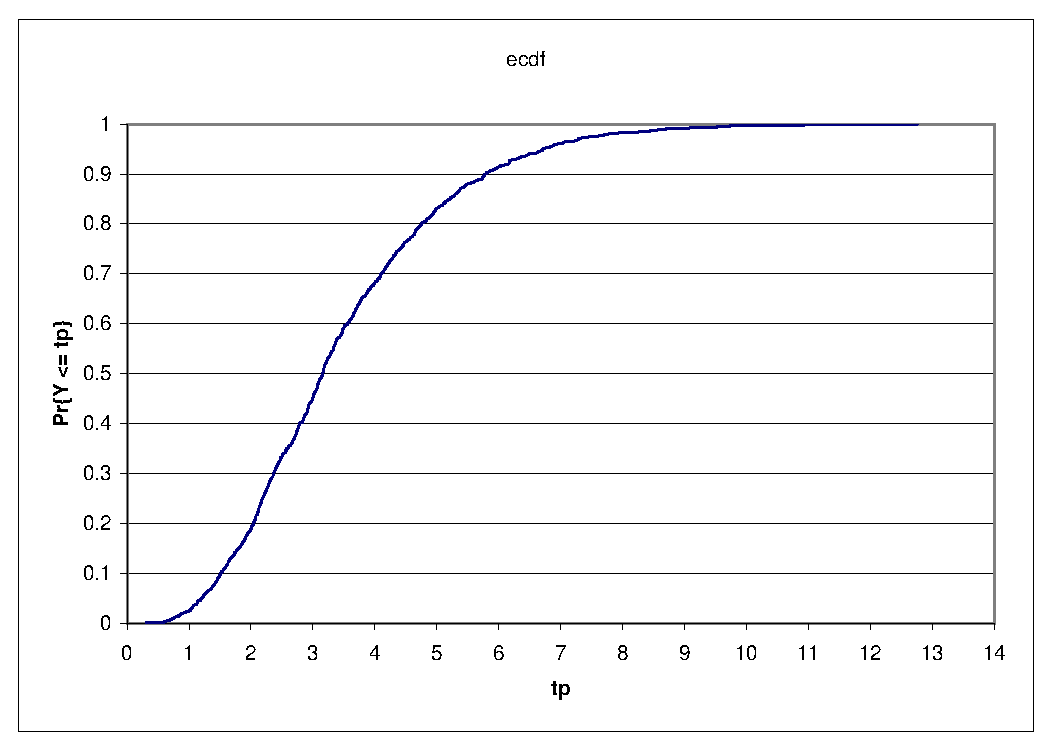
\includegraphics[width=4in]{figures/SANecdf}}
% \caption{Empirical cdf of the project completion times.}
% \label{fig:SANecdf}
% \end{figure}
% 
% Notice (see Fig.~\ref{fig:san.de.mainsimulation}) that the simulation ends
% when there are no additional activities remaining to be completed.
% 
% A difference between this implementation of the SAN simulation and the one in
% Sect.~\ref{sec:san.max.sim} is that here we write out the actual
% time the project completes on each replication. By doing so, we can
% estimate $\Pr\{Y > t_p\}$ for any value of $t_p$ by sorting the data
% and counting how many out of $1000$ replications were greater than
% $t_p$. Figure~\ref{fig:SANecdf} shows the empirical cdf of the $1000$
% project completion times, which is the simulation estimate
% of Eq.~(3.12).%~(\ref{eq:san.analytic}).
% 
% \subsection{Issues and Extensions}
% \label{sec:sim.san.issues}
% 
% \begin{enumerate}
% 
% \item In real projects there are not only activities, but also
% limited and often shared resources that are needed to complete the
% activities. Further, there may be specific resource allocation rules
% when multiple activities contend for the same resource. How might
% this be modeled in SimPy?
% 
% \item Time to complete the project is an important overall measure,
% but at the planning stage it may be more important to discover which
% activities or resources are the most critical to on-time completion
% of the project. What additional output measures might be useful for
% deciding which activities are ``critical?''
% 
% \end{enumerate}


\section{Simulating the Asian Option}
\label{sec:sim.asian}
\index{Asian option}


Here we consider estimating the value of an Asian option
\[
\nu = \E\left[ \mathrm{e}^{-rT} (\bar{X}(T) - K)^+ \right] 
\]
as described in Sect.~(3.5),%\ref{sec:fe}, 
where the maturity is $T = 1$
year, the risk-free interest rate is $r = 0.05$ and the strike price
is $K = \$55$. The underlying asset has an initial value of $X(0) =
\$50$ and the volatility is $\sigma^2 = (0.3)^2$.  Recall that the
key quantity is
\[
\bar{X}(T) = \frac{1}{T}\int_0^T X(t)\, \D t 
\]
the time average of a continuous-time, continuous-state geometric
Brownian motion 
process which we cannot truly simulate on a digital computer.
\index{geometric Brownian motion}
Thus, we approximate it by dividing the
interval $[0, T]$ into $m$ steps of size $\Delta t =
T/m$ and using the discrete approximation
\[
\widehat{\bar{X}(T)} = \frac{1}{m}
\sum_{i=1}^m X(i \Delta t) .
\]
This makes simulation possible, since 
\[
X(t_{i+1}) = X(t_i) \exp\left\{\left( r - \frac{1}{2}\sigma^2
\right)(t_{i+1}
- t_i) + \sigma\sqrt{t_{i+1} - t_i} \, Z_{i+1} \right\}
\]
for any increasing sequence of times $\{t_0, t_1, \ldots, t_m\}$, 
where $Z_1, Z_2, \ldots, Z_m$ are i.i.d.\ $\mathrm{N}(0,1)$. 

Figure~\ref{fig:asian.sim} is R code that uses $m=32$ steps in
the approximation, and makes $10{,}000$ replications to estimate
$\nu$. Discrete-event structure would slow execution without any
obvious benefit, so a simple loop is used to advance time. The value
of the option from each replication is saved to a list for
post-simulation analysis.

Note that this simulation uses the {\tt foreach} package. 
The {\tt foreach} construct is similar to using {\tt for} loops or the {\tt apply} family of functions as it allows for executing R code repeatedly over a list.
However, the {\tt foreach} package goes beyond that and supports parallel execution, which is used when running the R code across multiple processors/cores for multicore computers, or even multiple nodes when run on a computer cluster, instead of only using a single processor for all R operations.

The estimated value of $\nu$ is \$2.14 with a relative error of just over 2\%
(recall that the relative error is the standard error divided by the
mean). As the histogram in Fig.~\ref{fig:AsianHistogram} shows, the
option is frequently worthless (approximately 68\% of the time), but
the average payoff, conditional on the payoff being positive, is
approximately \$6.95.


\begin{figure}[tb]
\begin{center}
\begin{minipage}[t]{6in}\small
\begin{verbatim}
library(foreach)
Asianoption <- function(interestrate, sigma, steps, initialValue,
                strikePrice, maturity, aseed){
#  Asian Options simulation
  set.seed(aseed)
  sumx = 0.0
  x = initialValue
  interval = maturity/steps
  sigma2 = (sigma*sigma)/2.0
  for (j in 1:steps){
    z = rnorm(1, 0, 1)
    x = x * exp((interestRate - sigma2) * interval +
                     sigma * sqrt(interval) * z)
    sumx = sumx + x
  }
  value = (exp(-interestRate * maturity) * 
                  max(sumx / (steps) - strikePrice, 0))
  value
}
replications = 10000
initialSeed = 1234
maturity = 1.0
steps = 32
sigma = 0.3
interestRate = 0.05
initialValue = 50.0
strikePrice = 55.0
interval = maturity / steps
values <- c()
for (i in 1:replications){
  values <- c(values, Asianoption(interestRate, sigma, steps, initialValue,
                      strikePrice, maturity, i + initialSeed))
}
print(mean(values))
print(sd(values)/sqrt(replications))  # standard error
print(sd(values)/sqrt(replications)/mean(values))  
hist(values, breaks=30, main="Value of asian option \n over 10000 replications",
     xlab="Value",ylab="Occurances")
positivepayoff = values[values>0]
print(mean(positivepayoff))
print(length(positivepayoff))
\end{verbatim}
\end{minipage}
\end{center}
\caption{R Simulation of the Asian option problem.}
\label{fig:asian.sim}
\end{figure}


\begin{figure}[tb]
\centerline{\includegraphics[width=4in]{figures/AsianHistogram}}
\caption{Histogram of the realized value of the Asian option from
10{,}000 replications.}
\label{fig:AsianHistogram}
\end{figure}

\section{Case Study: Service Center Simulation}
\label{sec:fax}

This section presents a simulation case based on a project provided by
a former student. While still relatively simple, it is more complex
than the previous stylized examples, and the answer is not known
without simulating. The purpose of this section is to illustrate how
one might attack simulation modeling and programming for a realistic
problem.

\begin{example}[Fax Center Staffing] \label{ex:fax}

A service center receives faxed orders throughout the day,
with the rate of arrival varying hour by hour. The arrivals are
modeled by a nonstationary Poisson process with the rates
shown in Table~\ref{tab:fax.arrivals}. \index{nonstationary Poisson
process}

\begin{table}[tb]
\caption{Arrival rate of faxes by hour.}
\label{tab:fax.arrivals}
\begin{center}
\begin{tabular}{lc}\hline
\multicolumn{1}{c}{Time}&Rate (faxes/minute) \\\hline
8 AM--9 AM & 4.37 \\
9 AM--10 AM & 6.24 \\
10 AM--11 AM & 5.29 \\
11 AM--12 PM & 2.97 \\
12 PM--1 PM & 2.03 \\
1 PM--2 PM & 2.79 \\
2 PM--3 PM & 2.36 \\
3 PM--4 PM & 1.04 \\\hline
\end{tabular}
\end{center}
\end{table}


A team of Entry Agents select faxes on a first-come-first-served basis
from the fax queue. Their time to process a fax is modeled as normally
distributed with mean $2.5$ minutes and standard deviation $1$ minute.
There are two possible outcomes after the Entry Agent finishes
processing a fax: either it was a simple fax and the work on it is
complete, or it was not simple and it needs to go to a Specialist for
further processing.  Over the course of a day, approximately 20\% of
the faxes require a Specialist.  The time for a Specialist to process
a fax is modeled as normally distributed with mean $4.0$ minutes and
standard deviation $1$ minute.  

Minimizing the number of staff minimizes cost, but certain
service-level requirements much be achieved.  In particular, 96\% of
all simple faxes should be completed within $10$ minutes of their
arrival, while 80\% of faxes requiring a Specialist should also be
completed (by both the Entry Agent and the Specialist) within $10$
minutes of their arrival.  

The service center is open from 8 AM to 4 PM daily, and it is possible
to change the staffing level at 12 PM. Thus, a staffing policy
consists of four numbers: the number of Entry Agents and Specialists
before noon, and the number of Entry Agents and Specialists after
noon.  Any fax that starts its processing before noon completes
processing by that same agent before the agent goes off duty; and
faxes in the queues at the end of the day are processed before the
agents leave work and therefore are not carried over to the next day.

\end{example}

The first step in building any simulation model is deciding
what question or questions that the model should answer. Knowing the
questions helps identify the system performance measures that the
simulation needs to estimate, which in turn drives the scope and level
of detail in the simulation model.

The grand question for the service center is, what is the minimum
number of Entry Agents and Specialists needed for both time
periods to meet the service-level requirements?  Therefore, the
simulation must at least provide an estimate of the percentage of
faxes of each type entered within 10 minutes, given a specific staff
assignment.

Even when there seems to be a clear overall objective (minimize the
staff required to achieve the service-level requirement), we often
want to consider trade offs around that objective. For instance, if
meeting the requirement requires a staff that is so large that they
are frequently underutilized, or if employing the minimal staff means
that the Entry Agents or Specialists frequently have to work well past
the end of the day, then we might be willing to alter the
service requirement a bit.  Statistics on the number and the time
spent by faxes in queue, and when the last fax of each day is actually
completed, provide this information. Including additional measures
of system performance, beyond the most critical ones, makes the
simulation more useful.

Many discrete-event, stochastic simulations involve entities that
dynamically flow through some sort of queueing network where they
compete for resources. In such simulations, identifying the entities
and resources is a good place to start the model. For this service
center the faxes are clearly the dynamic entities, while the Entry
Agents and Specialists are resources. The fax machines themselves
might also be considered a resource, especially if they are heavily
utilized or if outgoing as well as incoming faxes use the same
machines. It turns out that for this service center there is a bank of
fax machines dedicated to incoming faxes, so it is reasonable to treat
the arrival of faxes as an unconstrained external arrival process.
This fact was not stated in the original description of the problem;
follow-up questions are often needed to fully understand the system of
interest.

Whenever there are scarce resources, queues may form. Queues are often
first-in-first-out, with one queue for each resource, as they are in
this service center. However, queues may have priorities,
and multiple queues may be served by the same resource, or a single
queue may feed multiple resources. Queueing behavior is often a
critical part of the model. 

When the simulation involves entities flowing through a network of
queues, then there can be two types of arrivals: arrivals from outside
of the network and arrivals internal to the network. Outside
arrivals are like those we have already seen in the $M(t)/M/\infty$ and
$M/G/1$ examples.  Internal arrivals are departures from one queue
that become arrivals to others. How these are modeled depends largely
on whether the departure from one queue is an immediate arrival to the
next---in which case the departure and arrival events are effectively
the same thing---or whether there is some sort of transportation
delay---in which case the arrival to the next queue should be
scheduled as a distinct event.
For the service center the arrival of faxes to the Entry
Agents is an outside arrival process, while the 20\% of faxes that
require a Specialist are internal arrivals from the Entry Agents to
the Specialists. 

Critical to experiment design is defining what constitutes a
replication. Replications should be independent and identically
distributed. Since the service center does not carry faxes over from
one day to the next, a ``day'' defines a replication. If faxes did
carry over, but all faxes are cleared weekly, then a replication might
be defined by a work week. However, if there is always significant
carry over from one day to the next, then a replication might have to
be defined arbitrarily.

The work day at the service center is eight hours;
however the staff does not leave until all faxes that arrive before 4
PM are processed. If we defined a replication to be exactly eight
hours then we could be fooled by a staffing policy that allows a large
queue of faxes to build up toward the end of the day, since the entry
of those faxes would not be included in our statistics. To model a
replication that ends when there is no additional work remaining, we
will cut off the fax arrivals at 4 PM and then end the simulation when
the event calendar is empty. This works because idle Entry Agents and
Specialists will always take a fax from their queue if one is
available.

Rather than walk through the Simmer code line by line, we will point
out some highlights to facilitate the reader's understanding of the
code.

Figure~\ref{fig:fax.global} shows the global declarations for the
service center simulation.


\begin{figure}[tbp]\small
\begin{verbatim}
#  Experiment data -------------------------
periodlength = 60.0
maxrate = 6.24
F <- list(
            maxTime = 1000,    # hours
            theseed = 9999,
            period = periodlength,
            nPeriods = 8,
            meanRegular = 2.5/periodlength,  # hours
            varRegular = 1.0/periodlength , # hours
            stdRegular = sqrt(1.0)/periodlength,  # per hour
            meanSpecial = 4.0/periodlength,  # hours
            varSpecial = 1.0/periodlength,  # hours
            stdSpecial = sqrt(1.0)/periodlength,  # per hour
            c = 4.0,
            numAgents = 15,
            numAgentsPM = 9,
            numSpecialists = 6,
            numSpecialistsPM = 3,
            maxRate = maxrate,
            aRate = c(4.37, 6.24, 5.29, 2.97, 2.03, 2.79, 2.36, 1.04),
            # per minute
            faxRate = 4.37,
            meanTBA = 1 / (maxrate * periodlength),  # hour
            pSpecial = 0.20
          )
\end{verbatim}
\caption{Global declarations for service center simulation.}
\label{fig:fax.global}
\end{figure}

\clearpage

The main program for the simulation is in Fig.~\ref{fig:fax.main}.
Of particular note are the \texttt{add\_resource}
statements defining \texttt{agents}, \texttt{agentspm}, \texttt{specialagents}, and \texttt{specialagentspm}. The monitors associated with these resources
will be used to obtain the fraction of regular and special faxes for both the morning and the afternoon that
are processed within the $10$-minute requirement by recording a $1$
for any fax that meets the requirement, and a $0$ otherwise. The mean
of these values is the desired fraction.

Also notice is the condition that ends the main simulation
loop:
\begin{center}
\texttt{run(until=1000)}
\end{center} 

Because the simulation ends well after the arrivals cease, any faxes still in the queue will be completed prior to the end of the simulation.
When the event calendar is empty, then there are no additional faxes to
process, and no pending arrival of a fax. This condition will only
hold after 4 PM and once all remaining faxes have been entered.

\begin{figure}[tbp]\small
\begin{verbatim}

envs <- lapply(1:100, function(i) {
    simmer("faxcenter") %>%
    add_resource("agents", F[['numAgents']]) %>%
    add_resource("specialagents", F[['numSpecialists']]) %>%
    add_resource("agentspm", F[['numAgentsPM']]) %>%
    add_resource("specialagentspm", F[['numSpecialistsPM']]) %>%
    add_generator("fax", fax, 
                  function() rexp(n=1,rate = (1/F[['faxRate']]))) %>%
    add_generator("Change arrival rate", changearrivalrate,
                  function () 1000) %>%
    run(until=1000)#F[['maxTime']])
})

arrivals <- get_mon_arrivals(envs[[1]], per_resource = T)

arrivals %>% count('resource')
\end{verbatim}
\caption{Main program and statistics reporting for service center simulation.}
\label{fig:fax.main}
\end{figure}

\clearpage

Figure~\ref{fig:fax.agents} includes the trajectory that faxes follow once they are generated 
 and this determine how they are routed to agents.
As faxes are routed, the simulation determines if they require special handling
after the regular agent is complete (\texttt{sample()}).

Later, in the \texttt{get\_mon\_arrivals}) function of the main program shown in Figure \ref{fig:fax.main},
will be used to both get the number of total faxes of this type, the number that waited less than 10 minutes before completing processing, and the fraction.

Ten replications of this simulation with a staffing policy of $15$
Entry Agents in the morning and $9$ in the afternoon, and $6$
Specialists in the morning and $3$ in the afternoon, gives $0.98 \pm
0.04$ for the fraction of regular faxes entered in $10$ minutes or
less, and $0.84 \pm 0.08$ for the special faxes. The ``$\pm$'' are
$95$\% confidence intervals. This policy appears to be close to the
requirements, although if we absolutely insist on $80$\% for the
special faxes then additional replications are needed to narrow the
confidence interval.

\begin{figure}[tbp]\small
\begin{verbatim}
fax <- trajectory("morningfax") %>%
  branch(function() sample(c(1, 2), 1,
                           prob = c(F[['pSpecial']], 1-F[['pSpecial']])),
         c(T, T),
         trajectory() %>%
           seize("specialagents", 1) %>%
           # do stuff here
           timeout(function() rnorm(n=1, 
                                    mean=F[['meanSpecial']], 
                                    sd = F[['stdSpecial']])) %>%
           release("specialagents", 1),
         trajectory() %>%
           seize("agents", 1) %>%
           # do stuff here
           timeout(function() rnorm(n=1, 
                                    mean=F[['meanRegular']], 
                                    sd = F[['stdRegular']])) %>%
           release("agents", 1))



changearrivalrate <- create_trajectory("changearrivalrate") %>%
                          timeout(1) %>%
                          set_attribute("faxRate", F[['aRate']][2]) %>%
                          timeout(1) %>%
                          set_attribute("faxRate", F[['aRate']][3]) %>%
                          timeout(1) %>%
                          set_attribute("faxRate", F[['aRate']][4]) %>%
                          timeout(1) %>%
                          set_attribute("faxRate", F[['aRate']][5]) %>%
                          timeout(1) %>%
                          set_attribute("faxRate", F[['aRate']][6]) %>%
                          timeout(1) %>%
                          set_attribute("faxRate", F[['aRate']][7]) %>%
                          timeout(1) %>%
                          set_attribute("faxRate", F[['aRate']][8])
\end{verbatim}
\caption{Processes for arriving agents.}
\label{fig:fax.agents}
\end{figure}


\clearpage 

\subsection{Issues and Extensions}
\label{sec:sim.fax.issues}

\begin{enumerate}

\item There are many similarities between the programming for this
simulation and the event-based simulation of the $M/G/1$ queue.



\item The fax entry times were modeled as being normally distributed.
However, the normal distribution admits negative values, which
certainly does not make sense. What should be done about this?
Consider mapping negative values to 0, or generating a new value
whenever a negative value occurs. Which is more likely to be realistic
and why?

\end{enumerate}

\section*{Exercises}
\addcontentsline{toc}{section}{Exercises}

\begin{enumerate}

\item For the hospital problem, simulate the current system in which the
receptionist's service time is well modeled as having an Erlang-$4$
distribution with mean $0.6$ minutes. Compare the waiting time to the
proposed electronic kiosk alternative. 

\item Simulate an $M(t)/G/\infty$ queue where $G$ corresponds to an
Erlang distribution with fixed mean but try different numbers of
phases. That is, keep the mean service time fixed but change the
variability. Is the expected number if queue sensitive to the
variance in the service time?

\item Modify the SAN simulation to allow each activity to have a
different mean time to complete (currently they all have mean time
$1$). Use a Collection to hold these mean times.

\item Try the following numbers of steps for approximating the value
of the Asian option to see how sensitive the value is to the step
size: $m=8, 16, 32, 64, 128$.

\item In the simulation of the Asian option, the sample mean of
10{,}000 replications was $2.198270479$, and the standard deviation
was $4.770393202$. Approximately how many replications would it take
to decrease the relative error to less than 1\%?

\item For the service center, increase the number of replications
until you can be confident that that suggested policy does or does not
achieve the $80$\% entry in less than $10$ minutes requirement for
special faxes.

\item For the service center, find the minimum staffing policy (in
terms of total number of staff) that achieves the service-level
requirement.  Examine the other statistics generated by the simulation
to make sure you are satisfied with this policy. 

\item For the service center, suppose that Specialists earn twice as
much as Entry Agents.  Find the minimum cost staffing policy that
achieves the service-level requirement. Examine the other statistics
generated by the simulation to make sure you are satisfied with this
policy. 

\item For the service center, suppose that the staffing level can
change hourly, but once an Agent or Specialist comes on duty they
must work for four hours. Find the minimum staffing policy (in
terms of total number of staff) that achieves the service-level
requirement.

\item For the service center, pick a staffing policy that fails to
achieve the service level requirements by $20$\% or more. Rerun the
simulation with a replication being defined as exactly 8 hours, but do
not carry waiting faxes over to the next day. How much do the
statistics differ using the two different ways to end a replication?


\item The function \verb+NSPP_Fax+ is listed below. This function
implements the thinning method described in
Sect.~\ref{sec:sim.mminf} for a nonstationary Poisson process with
piecewise-constant rate function. Study it and describe how it works.
\index{nonstationary Poisson process} \index{thinning}

\small
\begin{verbatim}
def NSPP_Fax(arrivalrate, MaxRate, NPeriods, periodlength, stream):
    '''  Non-stationary Poisson Process

    This function generates interarrival times from a 
    NSPP with piecewise constant arrival rate over a fixed time of 
    NPeriod time units

    arrivalrate - Array of arrival rates over a
                common length period
    MaxRate - The maximum value of ARate
    NPeriods - Number of time periods in ARate
    periodlength - time units between (possible) changes 
                    in arrival rate
    '''
    random.seed(stream)
    pthinning = [(1-hourlyrate/MaxRate) for hourlyrate in arrivalrate]
    t = 0.0
    arrivaltimes = []
    totaltime = NPeriods * periodlength
    while t < totaltime:
        deltat = random.expovariate(MaxRate)
        t = t + deltat
        if t < totaltime:
            pthin = pthinning[int(floor(t/periodlength))]
            uthin = random.random()
            if uthin > pthin:
                arrivaltimes.append(float(t)) 
                # add arrival since not thinned
    return arrivaltimes
\end{verbatim} 
\normalsize

\item  Beginning with the event-based $M/G/1$ simulation,
implement the changes necessary to make it an $M/G/s$ simulation (a
single queue with any number of servers). Keeping $\lambda = 1$ and
$\tau/s = 0.8$, simulate $s=1,2,3$ servers and compare the results.
What you are doing is comparing queues with the same service capacity,
but with $1$ fast server as compared to two or more slower servers.
State clearly what you observe.

\item  Modify the Simmer event-based simulation of the $M/G/1$
queue to simulate an M/G/1/$c$ retrial queue. This means that customers
who arrive to find $c$ customers in the system (including the customer
in service) leave immediately, but arrive again after an exponentially
distributed amount of time with mean \texttt{MeanTR}.  Hint: The
existence of retrial customers should not affect the arrival process for
first-time arrivals. 

\item  This problem assumes a more advanced background in
stochastic processes. In the simulation of the $M(t)/M/\infty$ queue
there could be a very large number of events on the event calendar: one
``Arrival'' and one ``Departure'' for \textit{each} car currently in the
garage. However, properties of the exponential distribution can reduce
this to no more than two events.  Let $\beta = 1/\tau$ be the departure
rate for a car (recall that $\tau$ is the mean parking time). If at any
time we observe that there are $N$ car in the garage (no matter how long
they have been there), then the time until the first of these cars
departs is exponentially distributed with mean $1/(N\beta)$. Use this
insight to build an $M(t)/M/\infty$ simulation with at most two pending
events, next arrival and next departure. Hint: Whenever an arrival
occurs the distribution of the time until the next departure changes, so
the scheduled next departure time must again be generated.


\item  The phone desk for a small office is staffed from 8 AM
to 4 PM by a single operator. Calls arrive according to a Poisson
process with rate 6 per hour, and the time to serve a call is uniformly
distributed between 5 and 12 minutes.  Callers who find the operator
busy are placed on hold, if there is space available, otherwise they
receive a busy signal and the call is considered ``lost.'' In addition,
10\% of callers who do not immediately get the operator decide to hang
up rather than go on hold; they are not considered lost, since it was
their choice. Because the hold queue occupies resources, the company
would like to know the smallest capacity (number of callers) for the
hold queue that keeps the daily fraction of lost calls under 5\%. In
addition, they would like to know the long-run utilization of the
operator to make sure he or she will not be too busy.  Use Simmer to
simulate this system and find the required capacity for the hold queue.
Model the callers using a generator and the operator as a resource. 
Use the functions \texttt{rexp} and \texttt{runif} for random-variate
generation.  Estimate the fraction of calls
lost (record a 0 for calls not lost, a 1 for those that are lost so that
the sample mean is the fraction lost). Use the statistics collected by a monitor to estimate the utilization. 


\item \label{ex:smp} Software Made Personal (SMP)
customizes software products in two areas: financial tracking and
contact management.  They currently have a customer support call
center that handles technical questions for owners of their software
from the hours of 8 AM to 4 PM Eastern Time.

When a customer calls they the first listen to a recording that asks
them to select among the product lines; historically 59\% are financial
products and 41\% contact management products. The number of customers
who can be connected (talking to an agent or on hold) at any one time is
essentially unlimited.  Each product line has its own agents. If an
appropriate agent is available then the call is immediately routed to
the agent; if an appropriate agent is not available, then the caller is
placed in a hold queue (and listens to a combination of music and ads).
SMP has observed that hang ups very rarely happen.

SMP is hoping to reduce the total number of agents they need by
cross-training agents so that they can answer calls for any product
line.  Since the agents will not be experts across all products, this
is expected to increase the time to process a call by about 5\%.  The
question that SMP has asked you to answer is how many cross-trained
agents are needed to provide service at the same level as the current
system.

Incoming calls can be modeled as a Poisson arrival process with a rate
of $60$ per hour.  The mean time required for an agent to answer a
question is $5$ minutes, with the actual time being Erlang-$2$ for
financial calls, and Erlang-$3$ for contact management calls.  The
current assignment of agents is $4$ for financial and $3$ for contact
management.  Simulate the system to find out how many agents are
needed to deliver the same level of service in the cross-trained system
as in the current system. 
\end{enumerate}


\begin{thebibliography}{99}

\bibitem{Nelson2013} Barry Nelson, {\em Foundations and Methods for Stochastic Simulation|}, Springer: Boston, MA, 2013.

\bibitem{rcoreteam2016a}  {R Core Team}, {\em R: A language and environment for statistical computing}, R Foundation for Statistical Computing, Vienna, Austria, https://www.R-project.org/, 2016.

\bibitem{rcoreteam2016b} {R Core Team}, {\em R Data Import/Export}, R Foundation for Statistical Computing, Vienna, Austria, https://cran.r-project.org/doc/manuals/r-release/R-data.html, 2016.

\bibitem{simmer2016} Bart Smeets, I\~naki Ucar, {\em simmer: Discrete-Event Simulation for R}, https://cran.r-project.org/web/packages/simmer/index.html, 2016.

\bibitem{wickham2009} Hadley Wickham, {\em ggplot2: Elegant Graphics for Data Analysis.} Springer-Verlag New York, 2009.

\bibitem{wickham2014} Hadley Wickham, {\em Tidy Data}, Journal of Statistical Software, Vol 59, No 10, 2014, doi: 10.18637/jss.v059.i10.

\bibitem{wickham2015} Hadley Wickham and Romain Francois, {\em dplyr: A Grammar of Data Manipulation}. R package version 0.4.3, https://CRAN.R-project.org/package=dplyr, 2015.



\end{thebibliography}

\end{document}
